% Un articolo scritto con LaTeX
\documentclass[10pt,a4paper,usenatbib]{article}
\usepackage[round]{natbib}
\usepackage[T1]{fontenc} % imposta la codifica dei font
\usepackage[utf8]{inputenc} % lettere accentate da tastiera
\usepackage[italian]{babel} % per scrivere in italiano
\usepackage{layaureo} % imposta i margini di pagina
\usepackage{url} % per scrivere gli indirizzi Internet
\usepackage{wrapfig}
\usepackage{booktabs} %per poter usare "\toprule, \midrule, \bottomrule"
\usepackage{amsmath}
\usepackage{amsfonts}
\usepackage{amssymb}
\usepackage{graphicx}
\usepackage{tocloft} 
\usepackage{pdfpages}

\newcommand*{\unit}[1]{\ensuremath{\mathrm{\,#1}}}                              % per poter usare il comando "\unit{}"; 
\newcommand{\fpath}{./Figs/}
\addto{\captionsitalian}{\renewcommand{\abstractname}{Introduzione}}

\begin{document}

\author{Alessandro Liberatore \and Luca Rickler}
\title{Simulazione dello sviluppo di uno sciame elettromagnetico in atmosfera}
\maketitle

\begin{abstract}
Scopo del seguente programma è la simulazione con metodo Monte Carlo dello sviluppo di uno sciame elettromagnetico in atmosfera. 
\\Tale sciame si può immaginare come prodotto dall'interazione di un raggio cosmico primario con gli elementi componenti l'atmosfera terrestre. Si dà la possibilità all'utente di scegliere la particella, e la sua energia, che darà inizio allo sciame (in particolare è possibile scegliere tra elettrone, positrone o raggio gamma in un intervallo di energie tra i $10^2\unit{MeV}$ ed i $10^8\unit{MeV}$). 
\\I risultati di tale simulazione possono essere confrontati con quelli di altre simulazioni presenti allo stato dell'arte. 
\end{abstract}

%\tableofcontents

\section{Sciami atmosferici}
Un raggio cosmico primario può generare una cascata di particelle secondarie. Questo sciame di particelle viene comunemente chiamato \textit{Extensive Air Showers} (EAS). In particolare questi sciami sono composti sia da una componente elettromagnetica che da una adronica. Nella presente simulazione, si focalizzerà l'attenzione sulla sola componente elettromagnetica generata da un elettrone o un positrone o un raggio gamma e considerata come particella primaria. 

\subsection{Sciami elettromagnetici}
Come detto, si può considerare uno sciame elettromagnetico come prodotto dall'interazione di un elettrone, positrone o raggio gamma con l'atmosfera terrestre. Date le alte energie in gioco ($\approx10^8\unit{MeV}$), i fenomeni di interazione predominanti per queste particelle a tali energie sono:
\begin{itemize}
\item \textbf{bremsstrahlung} per gli elettroni ed i positroni;
\item \textbf{produzione di coppia} per i raggi gamma.
\end{itemize}
Si supponga, a titolo di esempio, un elettrone come particella primaria. Si avrà la creazione di fotoni (per via della radiazione di bremsstrahlung) che possono a loro volta creare elettroni e positroni tramite la produzione di coppia che a loro volta potranno rifare bremsstrahlung e così via. Il processo continua fino al raggiungimento delle energie critiche. Le energie di soglia sono $88.05\unit{MeV}$ per la bremsstrahlung e $10\unit{MeV}$ per la produzione di coppia. 
\\L'energia critica per la bremsstrhalung si è ricavata facendo una media ponderata tra la media dell'energia critica di elettroni e positroni immersi in azoto molecolare, ossigeno molecolare ed argon (si veda Appendice A). Si è infatti considerata un'atmosfera composta da: $78\% N_2$, $21\% O_2$ ed $1\% Ar$. Le varie energie critiche di elettroni e positroni nei singoli elementi sono state prese dal \textit{Particle data book} (PDG 2016). Per quanto riguarda l'energia di soglia per la produzione di coppie, si è scelto il valore di energia per il quale questo tipo di interazione predominasse sugli altri. A tal fine si è ritenuto, come si può osservare nel grafico in \figurename~\ref{jpg:AttenuazioneFotoni}, che $100\unit{MeV}$ fosse una buona scelta. 
 \begin{figure} [h!]
\centering
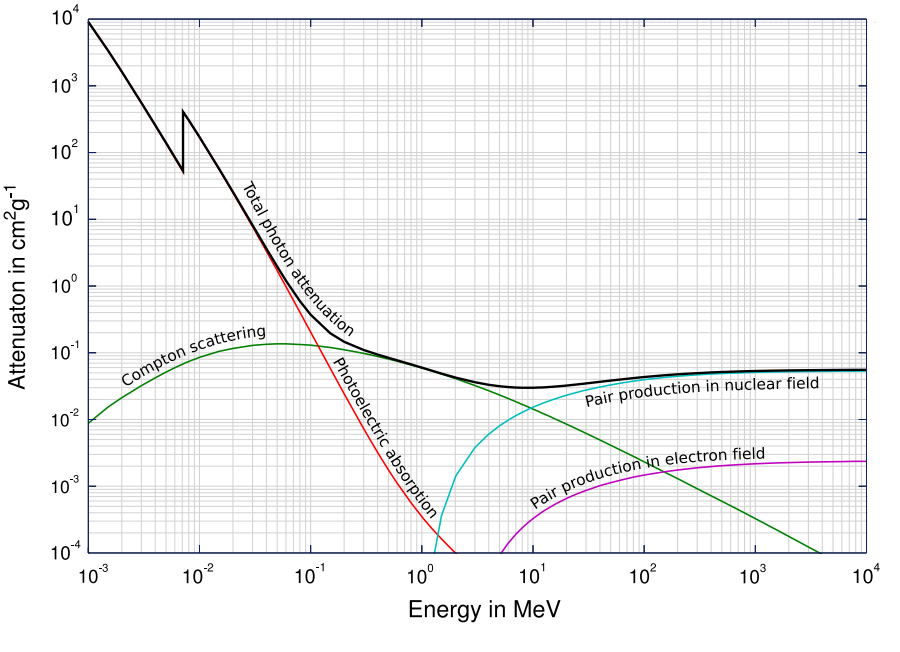
\includegraphics[width=11cm, height=11cm, keepaspectratio]{AttenuazioneFotoni}
\caption{Diversi meccanismi di attenuazione di fotoni in un mezzo in funzione dell'energia. }
\label{jpg:AttenuazioneFotoni}
\end{figure}
\\Si sono dunque considerate, fino al raggiungimento delle rispettive energie critiche, esclusivamente i processi di bremsstrahlung e di produzione di coppie (che portano allo sviluppo dello sciame). Successivamente, le singole particelle arrivano ad avere energie sotto soglia e, non creando nuove particelle, fanno cominciare il riassorbimento dello sciame. 
\\Viene spiegata di seguito, più in dettaglio, la logica utilizzata per la simulazione Monte Carlo dello sviluppo ed il riassorbimento dello sciame. 

\subsection{Sviluppo dello sciame}
Si consideri l'atmosfera come divisa in strati atmosferici di spessore pari ad una lunghezza di radiazione $\tilde{x}_0 \unit{[g/cm^2]}$. Nel primo strato atmosferico sarà presente il raggio cosmico primario che, se ad energia sufficiente, interagirà facendo produzione di coppia o bremsstrahlung. Studiamo separatamente il comportamento di elettroni/positroni e di raggi gamma. 
\\Cominciamo con il fenomeno di bremsstrahlung. Da letteratura (\textit{Passage of particles through matter}; January 2012, H. Bichsel, D.D. Groom, S.R. Klein), si trova che il numero di fotoni prodotti come radiazione di bremsstrahlung in funzione dello spazio percorso e dell'energia dei gamma emessi ($k_{min}$ e $k_{max}$) risulta essere pari a: 
\begin{equation}
N_\gamma = \frac{d}{\tilde{x}_0}\left[\frac{4}{3}\ln{\frac{k_{max}}{k_{min}}}-\frac{4(k_{max} - k_{min})}{3E_e}+\frac{k_{max}^2 - k_{min}^2}{2E_e^2}\right]
\end{equation}
che vale per distanze percorse $d \ll \tilde{x}_0 \unit{[g/cm^2]}$. Noto questo, si è proceduto estraendo casualmente un valore di energia tra $1 \unit{keV}$ ed $E_e$ (energia dell'elettrone/positrone generatore). Il valorore minimo è stato scelto arbitrariamente decidendo di ignorare i raggi gamma di energia inferiore al keV mentre il valore massimo è stato scelto uguale ad $E_e$ per una ovvia conservazione di energia. Da questa equazione, a fissata $E_e$, ricavo il libero cammino medio $d$ ponendo $N_\gamma = 1$ e $k_{min}$, $k_{max} = 1 \unit{keV}$, $E_e$. Il risultato, che ci dà quindi la distanza entro la quale ho per certo la produzione di un raggio gamma, lo si usa come coefficiente di una distribuzione esponenziale con coefficiente $d$ da cui si estrae randomicamente la distanza in cui consideriamo emesso il fotone. Ho quindi la distanza in cui viene emesso un $\gamma$ di bremsstrahlung di energia estratta, di nuovo randomicamente, tra $1\unit{keV}$ ed $E_e$. Bisogna ora valutare se questa energia estratta risulta superiore a $10\unit{keV}$ (ovvero è in grado di fare produzione di coppie). In caso affermativo, si genererà appunto un fotone di energia pari all'energia estratta e tolgo questa energia all'elettrone generatore. In caso contrario, non genero il fotone (che "morirà subito" in quanto non sarà in grado di fare neanche una volta produzione di coppia) ma conservo lo stesso l'energia sottraendo l'energia estratta per il fotone, all'energia dell'elettrone generatore. Questo processo si fà per ogni elettrone che si viene a creare nello sciame con energia suffiente per fare bremsstrahlung (energia che di volta in voltà andrà a diminuire) ed in ogni distanza estratta, come detto, casualmente da una distribuzione esponenziale di coefficiente $d$. 
\\I fotoni, invece, fanno creazione di coppia ad una distanza fissa pari a: 
\begin{equation}
x = \frac{7}{9}\tilde{x}_0. 
\end{equation}
come noto da manuali. 
\\Ad ogni creazione di coppia, l'energia del fotone viene esattamente divisa a metà tra l'elettrone ed il positrone creati. 
\\Ogni particella creata (sia gamma di bremsstrahlung che elettroni/positroni di produzione di coppia) sono stati considerati emessi ad un certo angolo zenitale $\theta$ e ad uno azimutale $\phi$ (variabile casualmente tra 0 e $2\pi$). L'angolo $\theta$ ha invece valore medio, tenuto costante, di: 
\begin{equation}
\langle\theta\rangle = \frac{m_e c^2}{E_e}
\end{equation}
per l'emissione dei gamma di bremsstrahlung, e di: 
\begin{equation}
\langle\theta\rangle = \frac{m_e c^2}{E_\gamma}
\end{equation}
per l'angolo rispetto la verticale per l'emissione di coppie. Conoscendo $\theta$ e conoscendo la distanza ($x$) percorsa dalle particelle, possiamo risalire allo step verticale ($s$) compiuto attraverso la trigonometria: $s = x\cos{\theta}$. 
\\Questi processi continuano, step dopo step, fino al raggiungimento delle rispettive energie di soglia. 

\subsection{Riassorbimento dello sciame}
Per quanto riguarda il riassorbimento dello sciame, si è proceduto nuovamente in modo diverso per elettroni/positroni e raggi gamma. 
\\Per quanto riguarda gli elettroni, una volta che hanno raggiunto valori di energia sotto soglia, percorrono uno strato atmosferico pari al range di percorrenza degli elettroni in un mezzo che, da letteratura (L. Katz and A.S. Penfold, \textit{Rev. Mod. Phys.}, 24 (1952), p.28.), risulta pari a: 
\begin{equation}
R_{max} = \begin{cases} 0.412 E_e^{1.265-0.0954 \ln{E_e}}     & 0.01\le E_e \le 2.5\unit{MeV} \\ 
                                          0.530 E_e - 0.106                                   & E_e > 2.5\unit{MeV}. 
                   \end{cases}
\end{equation}
I raggi gamma vengono invece subito abbandonati una volta sotto la soglia della produzione di coppia (non si considerano dunque effetti quali lo scattering Compton e l'effetto fotoelettrico). 

\section{Descrizione codice}


\section{Compilazione codice}


\section{Risultati e confronti con altri modelli}
%Come conferma della bontà della simulazione, si sono paragonati i risultati ottenuti con quelli di altre simulazioni. In particolare si può notare come l'andamento dell'energia per strato atmosferico ottenuto sia in linea con quello ottenuto con simulazioni svolte con Geant4 e come il coefficiente angolare ottenuto dallo studio dell'elongation rate sia effettivamente prossimo a quello stimato nel modelli di Heitler.% 

\pagebreak
\appendix
\section{Appendici}
\subsection{Calcolo dell'energia critica e della lunghezza di radiazione per elettroni e positroni in atmosfera}
Si consideri un'atmosfera composta da: $78\% N_2$, $21\% O_2$ ed $1\% Ar$. Dal \textit{Particle data book} (PDG 2016) si hanno i seguenti valori: 
\begin{table}[h!]
\centering
\begin{tabular}{lccc}
\toprule
                      &   $x_0$ [m]   &   $\tilde{x}_0$ [$\unit{g/cm^2}$]   &   $E_c$ [MeV]                  \\                          
\midrule
$N_2$:          &   326              &   37.99                               &  $e^-$: 91.74; $e^+$: 89.71        \\
$O_2$:          &   257              &   34.24                               &  $e^-$: 81.45; $e^+$: 79.62         \\
$Ar$:             &   118              &   19.55                               &  $e^-$: 38.03; $e^+$: 37.06          \\
\bottomrule
\end{tabular}
\end{table}
Da questi valori è possibile ricavare una lunghezza di radiazione $\tilde{x}_0$ ed una energia critica media per elettroni e positroni in atmosfera: \\
\begin{equation*}
\tilde{x}_0 = \frac{37.99*78+34.24*21+19.55*1}{78+21+1} \approx 37.02\unit{g/cm^2};
\end{equation*}
\\
\begin{equation*}
E_c = \frac{\frac{91.74 + 89.71}{2}*78+\frac{81.45 + 79.62}{2}*21+\frac{38.03 + 37.06}{2}*1}{78+21+1} \approx 88.05\unit{MeV};
\end{equation*}
\\che sono i valori che si utilizzano nella simulazione sia per gli elettroni che per i positroni. 

\bibliographystyle{plainnat}
\bibliography{sample}

\end{document}



%/////////////////////////////////////////////////////////////////////////////////////////////////////////////////////////////////////////////////////%



Lo sviluppo di uno sciame elettromagnetico si basa su due processi fondamentali è comunemente descritto, con le opportune approssimazioni e semplificazioni, dal modello di Heitler. 
\\Uno sciame E.M. è generato da un $\gamma$ o un $e^\pm$ che interagisce con l'atmosfera terrestre. La perdita di energia da parte di un $\gamma$ o un $e^\pm$ in atmosfera è descrivibile da: 
\begin{equation}
-\frac{dE}{d\xi} = \frac{E}{\lambda_T}
\end{equation}
da cui ottengo: 
\begin{equation}
E(\xi) = E_0 e^{- \xi/\lambda_T}
\end{equation}
con $\lambda_T$ dell'aria che vale $\approx 37\unit{g cm^{-2}}$. La quantità di materia attraversata dalla particella prima di perdere metà della propria energia è quindi data da: 
\begin{equation}
\frac{E(\xi)}{E_0} = \frac{1}{2} =  e^{- \xi/\lambda_T}
\end{equation}
da cui ottengo: 
\begin{equation}
\xi = \lambda_T \ln{2}. 
\end{equation}
Ciò significa che un $e^\pm$ emette, per bremsstrahlung, un $\gamma$ dopo avere percorso una distanza di dimezzamento $d = \lambda_T \ln{2}$. Un $\gamma$ dopo avere percorso la stessa distanza (in realtà sarebbe $\lambda_p = 9/7 \lambda_T$ ma approssimo $\lambda_p \approx \lambda_T$) dà origine ad una coppia elettrone positrone. 
\\Considero che, ad ogni interazione, l'energia dei $e^\pm$ (e dei $\gamma$) venga divisa \textit{a metà}. Queste sono tutte approssimazioni fatte per semplificare il modello. In \figurename~\ref{jpg:ModelloHeitler} è schematizzato lo sviluppo di uno sciame E.M. generato da un $\gamma$ primario interagente con l'atmosfera. 
\begin{figure} [h!]
\centering
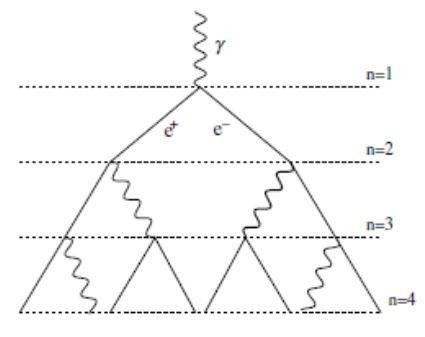
\includegraphics[width=11cm, height=11cm, keepaspectratio]{ModelloHeitler}
\caption{Sviluppo in atmosfera di uno sciame elettromagnetico generato da un $\gamma$ (dove "$n$" indica il numero di lunghezze di radiazione, considerate uguali per $e^\pm$ e $\gamma$, attraversate dallo sciame). }
\label{jpg:ModelloHeitler}
\end{figure}
\\Consideriamo uno sciame iniziato da un $\gamma$ di energia $E_0$. Dopo $n$ lunghezze di dimezzamento $d$ avremo $2^n$ particelle di energia $E_0/2^n$ l'una. 
\\Dunque lo spazio percorso dopo $n$ lunghezze di dimezzamento $d$ sarà: 
\begin{equation}
X = n d, 
\end{equation}
ma anche che:
\begin{equation}
 d = \lambda_T \ln{2}; 
\end{equation}
quindi otteniamo: 
\begin{equation}
 X = n \lambda_T \ln{2}; 
\label{eqn:profondità}
\end{equation}
che mi rappresenta appunto la profondità a cui mi arriva lo sciame. 
\\Poiché $\ln2 = \log_2{2}/\log_2{e}$, ho che il numero di particelle posso scriverlo come: 
\begin{equation}
 N = 2^n = 2^{X/(\lambda_T \ln2)} =  2^{\frac{X}{\lambda_T} \log_2{e}} = e^{\frac{X}{\lambda_T}}. 
\end{equation}
Il numero di particelle al massimo sviluppo dello sciame ($N_{max}$), considerando che la moltiplicazione termina quando l'energia delle particelle diventa inferiore dell'energia critica, è: 
\begin{equation}
\begin{cases}
N_{max} = 2^{n_{critico}} \\
E_0 = N_{max} E_{critico}^\gamma \\
\end{cases}
\end{equation}
da cui otteniamo: 
\begin{equation}
n_{critico} = \frac{1}{\ln2} \ln{\frac{E_0}{E_{critico}^\gamma}} 
\label{eqn:ncritico}
\end{equation}
e, di conseguenza, si ha che: 
\begin{itemize} 
\item \textbf{Numero particelle al massimo sviluppo dello sciame:} $N_{max} \propto E_0$; 
\item  \textbf{Profondità di massimo sviluppo:} $X_{max} \propto \ln(E_0)$; 
\end{itemize}
dove la proporzionalità per la profondità di massimo sviluppo si trova sostituendo alla~(\ref{eqn:profondità}) il valore di $n_{critico}$ trovato in~(\ref{eqn:ncritico}). 
\\Tuttavia raramente gli esperimenti si trovano esattamente al massimo sviluppo di uno sciame. Trovandosi più in basso del massimo dello sciame, misuro principalmente il numero di elettroni presenti in esso. Si trova che il modello descritto sovrastima il numero di elettroni rispetto quello dei $\gamma$. Si introduce quindi una costante di attenuazione $g=10$: 
\begin{equation}
N_e = \frac{N_{max}}{g}. 
\label{eqn:gNe}
\end{equation}
\\Sperimentalmente si misura anche la così detta \textit{elongation rate} che è definita come la crescita di $X_{max}$ \textit{in funzione di $E_0$}:  
\begin{equation}
\Delta \equiv \frac{dX_{max}}{d\log{E_0}} 
\end{equation}
e poiché, come visto, ho che: 
\begin{equation}
X_{max} = \lambda_T \ln{10} \log{\frac{E_0}{E_{critico}^\gamma}}
\label{eqn:Xmax}
\end{equation}
(dove ho usato: $\log_{10}{\frac{E_0}{E^\gamma}} = \frac{\ln{(E_0/E^\gamma)}}{\ln{10}}$), ottengo: 
\begin{equation}
\begin{split}
\Delta &= \frac{dX_{max}}{d\log{E_0}} \\
&= \frac{d(\lambda_T \ln{10} \log{(E_0/E^\gamma_{critico})})}{d\log{E_0}} \\
&= \frac{d(2.3\lambda_T (\log{E_0} - \log{E^\gamma_{critico})})}{d\log{E_0}} \\
&= 2.3\lambda_T. 
\end{split}
\end{equation}
Osserviamo quindi che il valore dell'\textit{elongation rate} (che ricordiamo essere la variazione di $X_{max}$ \textit{in funzione di $E_0$}) è circa \textit{costante}! Rappresentando quindi $X_{max}$ in funzione del logaritmo in base dieci dell'energia del primario, mi aspetto di ottenere una retta con coefficiente angolare circa pari a 2.3. 









